\documentclass[conference]{IEEEtran}
\IEEEoverridecommandlockouts
% The preceding line is only needed to identify funding in the first footnote. If that is unneeded, please comment it out.
\usepackage{cite}
\usepackage{amsmath,amssymb,amsfonts}
\usepackage{algorithmic}
\usepackage{graphicx}
\usepackage{textcomp}
\usepackage{xcolor}
\usepackage[caption=false, font=footnotesize]{subfig}
\def\BibTeX{{\rm B\kern-.05em{\sc i\kern-.025em b}\kern-.08em
    T\kern-.1667em\lower.7ex\hbox{E}\kern-.125emX}}
\begin{document}

\title{Estimating Subgraph Generation Models}

\author{\IEEEauthorblockN{1\textsuperscript{st} Laurens Bogaardt}
\IEEEauthorblockA{\textit{Netherlands eScience Center} \\
Amsterdam, the Netherlands \\
l.bogaardt@esciencecenter.nl}
\and
\IEEEauthorblockN{2\textsuperscript{nd} Frank Takes}
\IEEEauthorblockA{\textit{University of Amsterdam}\\
Amsterdam, the Netherlands\\
takes@uva.nl}
}

\maketitle

\begin{abstract}
Lorem ipsum dolor sit amet, consectetur adipiscing elit, sed do eiusmod tempor incididunt ut labore et dolore magna aliqua. Ut enim ad minim veniam, quis nostrud exercitation ullamco laboris nisi ut aliquip ex ea commodo consequat.
\end{abstract}

\begin{IEEEkeywords}
Networks, Graphs, ERGM, SUGM, Subgraphs
\end{IEEEkeywords}

\section{Introduction}

Lorem ipsum dolor sit amet, consectetur adipiscing elit, sed do eiusmod tempor incididunt ut labore et dolore magna aliqua~\cite{Chandrasekhar2014}.
Lorem ipsum dolor sit amet, consectetur adipiscing elit, sed do eiusmod tempor incididunt ut labore et dolore magna aliqua.
Lorem ipsum dolor sit amet, consectetur adipiscing elit, sed do eiusmod tempor incididunt ut labore et dolore magna aliqua.
Lorem ipsum dolor sit amet, consectetur adipiscing elit, sed do eiusmod tempor incididunt ut labore et dolore magna aliqua.

\section{Subgraph Generation Model}

Lorem ipsum dolor sit amet, consectetur adipiscing elit, sed do eiusmod tempor incididunt ut labore et dolore magna aliqua.
Lorem ipsum dolor sit amet, consectetur adipiscing elit, sed do eiusmod tempor incididunt ut labore et dolore magna aliqua.
Lorem ipsum dolor sit amet, consectetur adipiscing elit, sed do eiusmod tempor incididunt ut labore et dolore magna aliqua.

The observed network (left in Fig.~\ref{fig:Figure02}) is the union of all subgraphs (right in Fig.~\ref{fig:Figure02}), where the generated subgraphs may overlap. Multiple subgraphs may incidentally form additional structures such as triangles or squares.

\begin{table}[h!]
\def\arraystretch{1.6}
\caption{Probabilities in the Subgraph Census}
\begin{center}
\begin{tabular}{|c|c|c|c|c|}
\hline
\textbf{}&\multicolumn{4}{|c|}{\textbf{Subgraphs}} \\
\cline{2-5}
\textbf{Model}&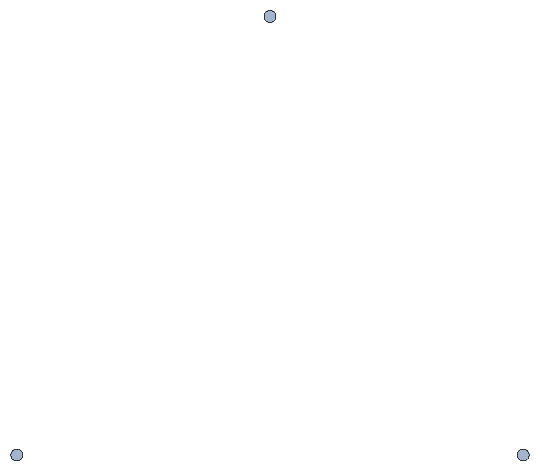
\includegraphics[scale=.2]{Figure03_1.pdf}&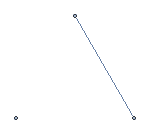
\includegraphics[scale=.2]{Figure03_2.pdf}&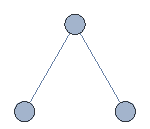
\includegraphics[scale=.2]{Figure03_3.pdf}&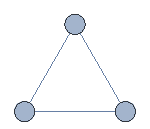
\includegraphics[scale=.2]{Figure03_4.pdf}\\
\hline
Links & $p_{L}^{3}$ & $3 \, p_{L}^{2} \, (1-p_{L})$ & $3 \, p_{L} \, (1-p_{L})^{2}$ & $(1-p_{L})^{3}$ \\
\hline
Triangles & $p_{T} \, (p_{T}^{n - 3})^{3}$ & $3 \, p_{T} \, (p_{T}^{n - 3})^{2} \, (1 - p_{T}^{n - 3})$ & $3 \, p_{T} \, (p_{T}^{n - 3}) \, (1-p_{T}^{n - 3})^{2}$ & $(1 - p_{T}) + p_{T} \, (1 - p_{T}^{n - 3})^{3}$ \\
\hline
Links \& Triangles & $p_{T} \, (p_{L} \, p_{T}^{n - 3})^{3}$ & $3 \, p_{T} \, (p_{L} \, p_{T}^{n - 3})^{2} \, (1 - p_{L} \, p_{T}^{n - 3})$ & $3 \, p_{T} \, (p_{L} \, p_{T}^{n - 3}) \, (1 - p_{L} \, p_{T}^{n - 3})^{2}$ & $(1 - p_{T}) + p_{T} \, (1 - p_{L} \, p_{T}^{n - 3})^{3}$ \\
\hline
\end{tabular}
\label{tab1}
\end{center}
\end{table}

\begin{figure}[htbp]
\begin{center}
\captionsetup[subfigure]{width=40mm}
\subfloat{\label{fig:Figure02_1.pdf}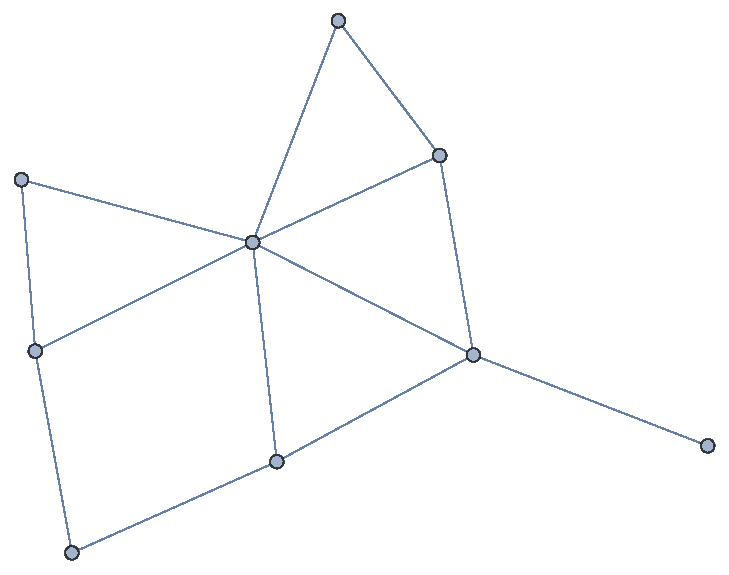
\includegraphics[scale=.35]{Figure02_1.pdf}}
\hfill
\subfloat{\label{fig:Figure02_1.pdf}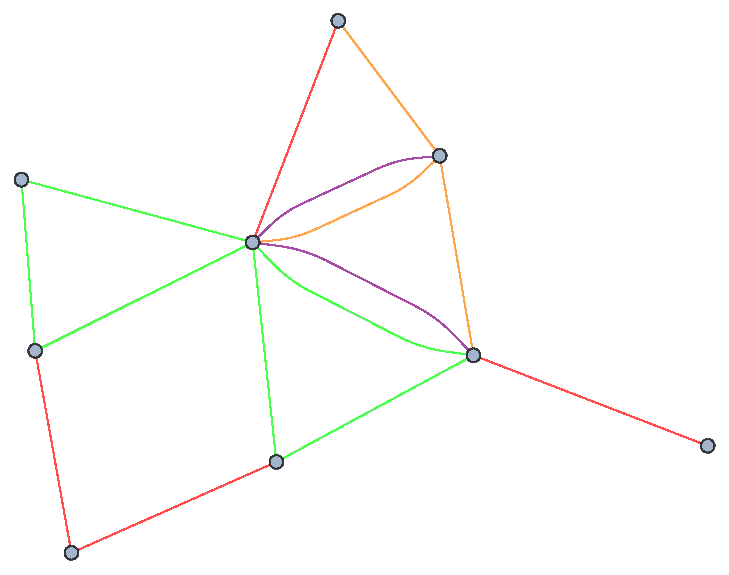
\includegraphics[scale=.35]{Figure02_2.pdf}}
\caption{The observed network (left) and the underlying, randomly generated links (red), 2-paths (purple), triangles (green) and 3-stars (yellow).}
\label{fig:Figure02}
\end{center}
\end{figure}

Lorem ipsum dolor sit amet, consectetur adipiscing elit, sed do eiusmod tempor incididunt ut labore et dolore magna aliqua.
\begin{equation}
f(x_{1}, \cdots, x_{k} ; p_{1}. \cdots, p_{k}) = \frac{\Gamma(\sum_{i} x_{i}+1)}{\prod_{i} \Gamma(x_{i}+1)} \prod_{i=1}^{k} p_{i}^{x_{i}}
\end{equation}

Lorem ipsum dolor sit amet, consectetur adipiscing elit, sed do eiusmod tempor incididunt ut labore et dolore magna aliqua.

\section{Further Research}

Lorem ipsum dolor sit amet, consectetur adipiscing elit, sed do eiusmod tempor incididunt ut labore et dolore magna aliqua.

\bibliographystyle{IEEEtran}
\bibliography{Bibliography}

\end{document}
